\section{Case Study}
In this section, we demonstrate the effective of our method with two real-world datasets.

\begin{figure}[htbp]
\centering
  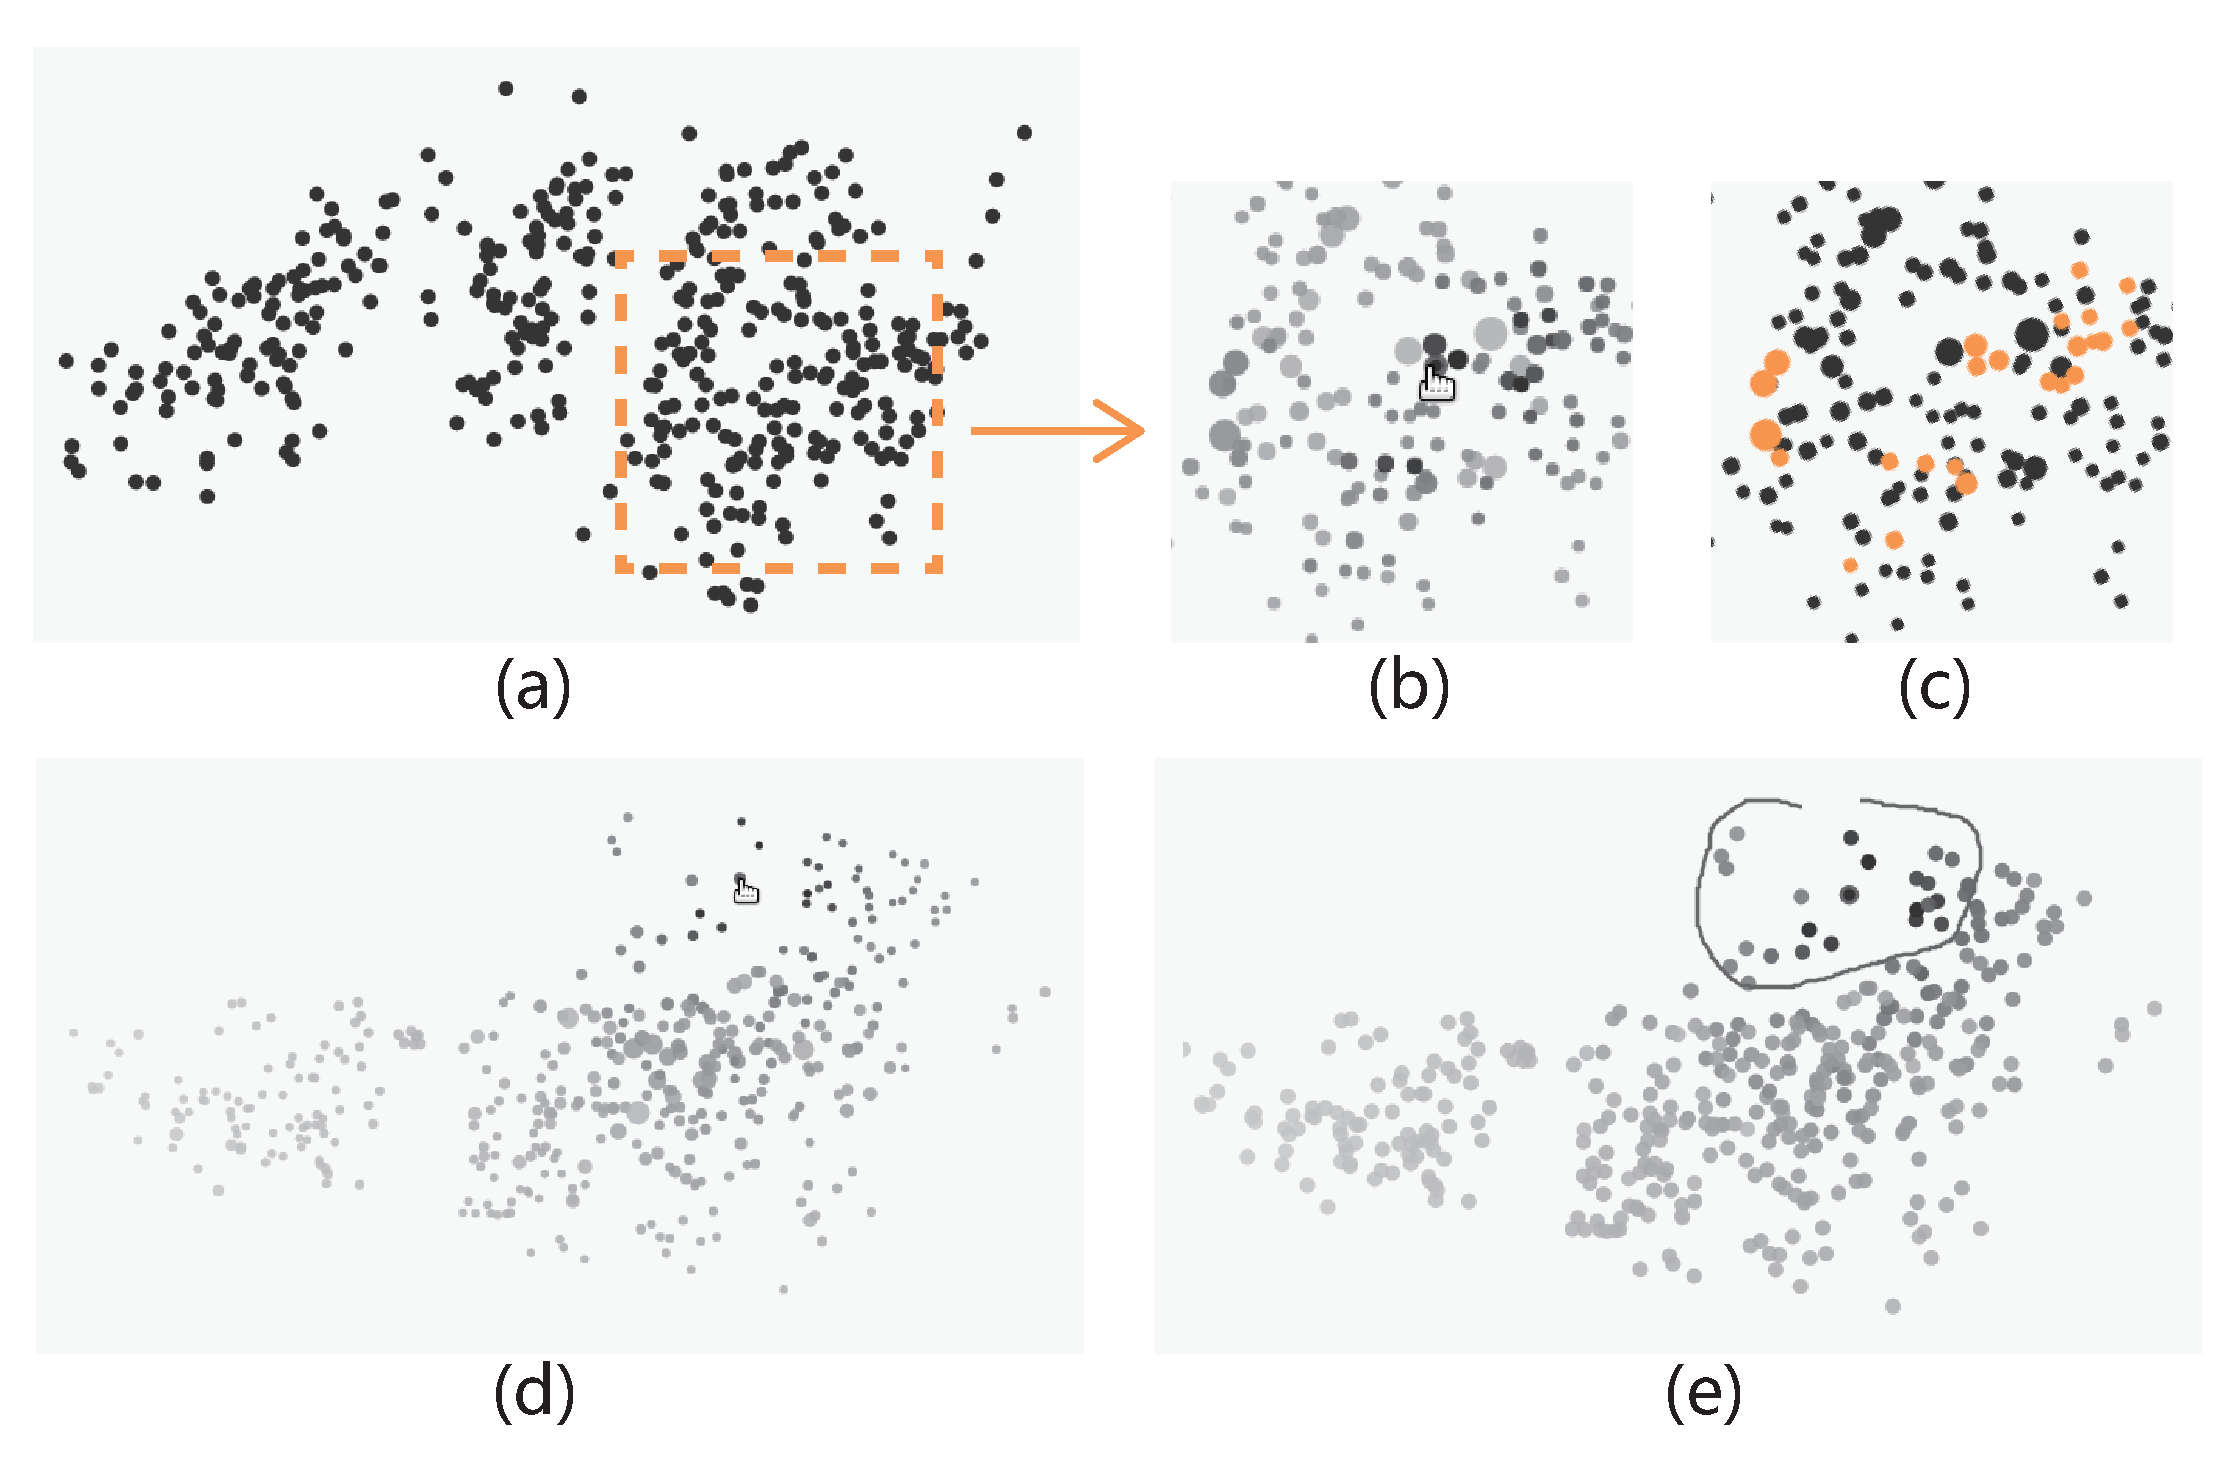
\includegraphics[width=1\linewidth]{images/case.eps}% 1\linewidth
  \caption{Car Data: Reducing local distortion}
\label{fig:car}
  \end{figure}

\begin{figure*}[htbp]
\centering
  \includegraphics[width=1\linewidth]{images/img_1.eps}% 1\linewidth
  \caption{USDA Food Data: First-level local analysis}
\label{fig:food1}
  \end{figure*}

\begin{figure*}[htbp]
\centering
  \includegraphics[width=1\linewidth]{images/img_2.eps}% 1\linewidth
  \caption{USDA Food Data: Second-level local analysis}
\label{fig:food2}
  \end{figure*}

\begin{figure*}[htbp]
\centering
  \includegraphics[width=1\linewidth]{images/img_3.eps}% 1\linewidth
  \caption{USDA Food Data: Third-level local analysis}
\label{fig:food3}
  \end{figure*}

\subsection{USDA Food Data}
The first case comes from the USDA Food Composition Data Set (http://www.ars.usda.gov/).  The dataset describes nutrients of a collection of raw or processed foods. It has been used in some previous works~\cite{DBLP:conf/ieeevast/TatuMFBSSK12}~\cite{DBLP:journals/tvcg/YuanRWG13} for their case studies. However, their methods focus on subspace mining, while we concern more about analyzing a piece of local data. After preprocessing, the dataset contains 722 records and 18 dimensions.

As shown in the overview (Figure~\ref{fig:food1}(a)), there are roughly three projection clusters. We choose one as the focus, aiming to analyze what foods it may contain. We use the Expand projection to see its inner structures (Figure~\ref{fig:food1}(b)). There seem to be some pattern, but not so obvious. We seek for the subspace suggestion with the threshold $R$ being $0.75$. The threshold keeps unchanged in the following process. Within the suggested subspace, we can see a more clear separation between a large  cluster and some outliers (Figure~\ref{fig:food1}(c)). In fact, the outliers include two tiny clusters, dominating two dimensions (Vitamin D and Sodium) respectively. Turning back to the overview, we find that the outliers are scattered all over the local region (Figure~\ref{fig:food1}(f)). It's hard to recognize and remove them without our local projection. So far, it is the first-level local analysis.

Then we go into the large cluster, to study the second-level locality. The cluster is extracted from the focus using the Decrease mode. In the Compress projection (Figure~\ref{fig:food2}(c)), a three-dimensional subspace is suggested. It shows that cluster members generally contain much energy and water, but have lower carbohydrate than the others. No matter what foods they are, they are unlikely grains. The subspace gets a score of 0.88, implying that the feature is rather obvious. The Expand projection (Figure~\ref{fig:food2}(b)) has four suggested dimensions: Vitamin D, Vitamin B6, Vitamin A and Vitamin B12. The focus is divided into three smaller clusters, each dominating one or two dimensions.

The first cluster (Figure~\ref{fig:food2}(d)) scores high in Vitamin D and Vitamin B6. They are probably not vegetables and fruits, which are poor in Vitamin D. The Compress projection (Figure~\ref{fig:food2}(g)) degrades to a 2D plane without using subspace suggestion. It's a strong pattern that none of the members has any fiber or beta carotene. This confirms our previous guess. Hence, we come to a primary conclusion: this cluster are probably fishes or dairy products, which are rich in Vitamin D and Vitamin B6.

The second cluster (Figure~\ref{fig:food2}(d)) scores high in Vitamin A, which is a property of animal livers. But it's also relatively low in Vitamin D, B6 and B12. This is a feature of plant-based foods. Most unselected data (colored in gray) behave similarly. Since the featured projection (Figure~\ref{fig:food2}(h)) did not give further information, we simply assume the cluster to be vegetables or animal livers. Back in the overview (Figure~\ref{fig:food2}(j)), these data are very close to the unselected data, which coincides with the local observation.

The third cluster seems rich in Vitamin B12. We enhance its inner relationships, going down to a third-level analysis. Again, there is one big cluster with some outliers in the projection (Figure~\ref{fig:food3}(b)). We remove the outliers, and enhance similarities within the cluster. The Compress view (Figure~\ref{fig:food3}(d)) shows a strong pattern that no fiber or Vitamin C exists here. The subspace score reaches 0.99. We can safely conclude that these are animal-based foods. In the Expand projection (Figure~\ref{fig:food3}(c)), five dimensions are suggested. The data are very diverse along the axis of lipid, while they separate into two groups in the other four dimensions. They are possibly fishes or red meats. In the overview, the two clusters are very close, yet separable (Figure~\ref{fig:food3}(g), (h)).

In the above process, we have found outliers and hierarchical clusters in different levels of locality. The four clusters seem layered in the overview(Figure~\ref{fig:food2}(i), (j), Figure~\ref{fig:food3}(g), (h)). Without the featured local projections, it's hard for users to discover and interpret those clusters. Besides, the projections also help to understand the unselected data, and how the focus resembles or differs from them. This will be impossible if the context data are discarded in the projection.

\label{section:casestudy}